\section{Introduction}
\label{sec:intro}

Observational sciences such as astronomy have long relied on computing \todo{computational resources} to extract scientific discoveries from measurements. Since
cause and effect cannot be studied directly\todo{in the field of astronomy?} with controlled experiments, expert analysis
of\todo{observational data from astronomical instruments} data is the only way that processes which cannot be interacted with can be
understood. 

This is true in the field of heliophysics whose goal is to understand the sun\todo{Sun} and its interactions with Earth and the solar system, including space weather. This field includes\todo{combines} a number of sub-disciplines such as solar physics, ionospheric and magnetospheric physics. The only way to make significant progress in understanding the fundamental processes in this complex system requires that interconnections be made across traditional science disciplines.\todo{suggested reword: In order to advance our understanding of the fundamental processes underpinning this complex system, interdisciplinary research across these scientific disciplines are required.} This \todo{however}is made difficult by the diversity of data sets involved. At the time of writing, NASA alone operates 18 missions with 24 spacecraft with 5 missions current under development as part of its Heliophysics Systems Observatory.  Software packages to analyze these datasets have generally been developed by the projects that designed and built the observatories through direct funding. These packages have provided some level of documentation and user support with various levels of quality. The result of this approach is a diverse and therefore difficult data environment to traverse.A common platform that addresses simple tasks, provides a standardize interface to data products, and encourages re-use of common functions can go a long way toward solving this problem. SunPy is a project which aims to solve this problem for the field of solar physics. \todo{the problem needs to be properly defined - i.e. difficult for users, no common platform, non-consistent, producibility etc.}

The primary goal of the SunPy Project is to facilitate and promote the use and development of a community-led, free and open-source data-analysis software based on the scientific \python\footnote{\url{https://www.python.org/}} environment.\todo{remove sentance of last paragraph as restated here.} To achieve that goal the project develops and maintains a core package (\sunpypkg) and supports an ecosystem of affiliated packages that provide additional functionality built on top of the core package. The project was formally founded in March of 2014. Development of the core package began three years earlier. Version 0.5, which was released on Jun 2014. was described in \citep{Community:2015cy}.
\todo{define open source with a link to https://opensource.org/osd}

The project began as a community-led effort to organize and standardize existing functionality and also to provide a \todo{Would "open source" be better than "free" because SSW is "free" but it's not "open source" - SJM} free and modern alternative to the existing SolarSoft (SSW, \citet{Freeland:1998we}) software package. While SSW is open source and freely available, it is primarily composed of source code for the Interactive Data Language (IDL), a proprietary data-analysis environment currently owned by Harris Geospatial Solutions. In addition, the development of SSW is not open to the community and is not version controlled.

The SunPy project has chosen \package{Python} to leverage the rich ecosystem of packages available for general scientific analysis. These include packages such as
\package{Numpy} which provides efficient multi-dimensional numerical array manipulation \citep{numpy} ; \package{scipy} which provides fundamental scientific functions such as for numerical integration and optimization\citep{scipy}; \package{Matplotlib} provides publication-ready 2D plotting \citep{matplotlib}, and finally \package{Pandas} provides data structures and analysis support with support for time series \citep{pandas}. These packages form the foundation of the scientific \python ecosystem. Together they represent $>$500,000 lines of code\footnote{As measured by cloc (\url{github.com/AlDanial/cloc})}. Significant packages have been built on top of these foundations. Of particular relevance to \sunpypkg is the \package{Astropy} package which provides common core functionality for astronomy \citep{astropy2018}. 

%NumPy 102906 LOC
%SciPy 139009 LOC
%matplotlib 98720 LOC
%pandas 212338 LOC
%astropy 151825 LOC

%The SunPy Project aims to develop and provide high-quality, maintainable and tested code paired with extensive documentation that follow current best practices in software development. 

%The core library sets a standard and example for other codes to follow.

%A description of the current affiliated packages can be found in Section~\ref{sec:affil_packages}.

\section{Project Organization \& Enhancement Proposals - Steven Christe}
The \sunpy project has defined a formal mechanism to define itself as well as to propose significant changes to the project or to the core package. These proposals are referred
to as \sunpy Enhancement Proposals (SEPs) and are modeled after the Python Enhancement Proposal process. SEPs are used to define the project, the leadership structure, decision-making mechanisms, as well as propose new features for the \sunpypkg package. There are generally three types of SEP. 
\begin{itemize}
    \item \textbf{Standard}: Introduces and describes a new feature or changes to an existing feature (e.g. API change) and is meant to function as a high-level design document.
    \item \textbf{Process}: This type of SEP describes a new process or a change to an existing process in the management of the project. Examples include procedures, guidelines, changes to the decision-making process or management structure, and changes to the tools or environment.
    \item \textbf{Informational}: Provides information and does not introduce any new features or changes nor describes a new process.
\end{itemize}
The first two SEPs (SEP-0001 and SEP-0002) define themselves as well as the \sunpy project organization. They are version controlled and publicly available on \github\footnote{\url{https://github.com/sunpy/sunpy-SEP}}. The organization is designed similar to a non-profit with a board and an executive director. The board is composed of up to 10 community members who are elected by the board. The board also elects the executive director who is also referred to as the lead developer. The responsibilities of the lead developer include leading the developer community, providing user support, implementing new SEPs, developing and maintaining the core package, as well as supporting the development of affiliated packages. The lead developer is supported by a deputy as well as other volunteers from the developer community. Members of the board are elected to serve two year terms while the Lead Developer\todo{capitalized here an not before - which is correct?} serves one year long terms. This choice of structure is enable significant community involvement in the leadership of the project.

As of the time of writing, there are a total of 8 SEPs. Some notables SEPs have lead to the adoption of physical units throughout the code base (SEP-0003, see Section~\ref{sec:units}), defined the affiliated package program (SEP-0004, see Section~\ref{sec:affil_package}), standardized the use of coordinate and coordinate transformations (SEP-0005, see Section~\ref{sec:coords}), and led to the adoption of a high precision scientific time format (SEP-0008).

\section{Support \& Sustainability}
The \sunpy project has not received any significant direct financial support for its work facilitating and promoting open-source and open development software including developing \sunpypkg. Some development\todo{sdc - point to a list of all students, isn't this available on sunpy.org?} was funded by the Google Summer of Code (GSOC) and the ESA Summer of Code in Space (SOCIS) as well as a small grant (of 3,000 USD) from NumFOCUS. Aside from these competitive programs, the \sunpy project relies largely on unpaid, volunteer efforts from early-career scientists which donate their time sometimes as part of their regular work duties. Further, these developers receive little to no formal recognition for their work \citep{Muna2016}. This situation is similar to that faced by the \astropy project \citep{PriceWhelan:2018ji}. The \sunpy project is actively searching for appropriate funding models to support long-term sustainability. 

The National Academies of Sciences, Engineering, and Medicine's 2018 report on Open Source Software Policy Options for NASA Earth and Space Sciences \citep{NAP2018} outlines several solutions to alleviate this problem -- namely that the NASA Science Mission Directorate provide funding for new and existing open source software projects, promote scientists who spend time developing and improving open source software projects, and offer prizes for exemplary contributions to the open source software community. The \sunpy community supports solutions like these for all relevant funding agencies and furthermore has the ability to accept financial contributions from institutions or individuals through the NumFOCUS organization.

\section{Development Model - NABIL}

As the aim of Sunpy is to be a community-developed library, designed and developed for and by the solar physics community, we have an open development model. 
The \verb|sunpy core| package is hosted online by \href{http://github.com}{GitHub} at \url{https://github.com/sunpy/sunpy}.
This means that the entire codebase can be read and scrutinized by anyone and everyone and can suggest improvements or submit changes that will be released to all SunPy users at a future time.
Furthermore, the codebase is licensed under a permissive 2-clause BSD licence, therefore anyone can redistribute, improve, repackage or use it in a closed environment without fear of legal notices as long as the copyright notice and the license disclaimer about the warranty are maintained.

Since the codebase is on \href{http://github.com}{GitHub}, this means that we use Git (\url{https://git-scm.com/}) as its distributed version control software. This means that all changes, no matter how small are tracked and saved into a history that allows us to see how the codebase develops, enables an iterative development approach and allows us to revert changes if they are deemed to be no longer unnecessary or causes a bug in the future.

We strive to  maintain a high quality codebase and with that in mind we have set several rules to achieve this.

1. We follow several commonly used and widespread style guides so that our code and documentation are consistent in our codebase.
2. We require that all new features added will be documented in at least two of the following ways: code comments, formal documentation and gallery examples.
3. We require all new features or additions have corresponding test code that ensures the correct behaviour. While the entire codebase does not have 100\%, we are working towards that goal.
4.  All code changes are reviewed by the community before they are accepted into the codebase. It does not matter who submits the changes.  This is to ensure that no code is accepted blindly and also encourages are more critical view of our codebase. 

This development model is widely used within the scientific Python  community and is the most common model used by a wide variety of other projects, whether they are open or closed source and even proprietary software creators.

Additionally, SunPy makes use of "continuous integration" services which is explained in Section (Link me).

\begin{figure}
\begin{tabular}{ccc}
  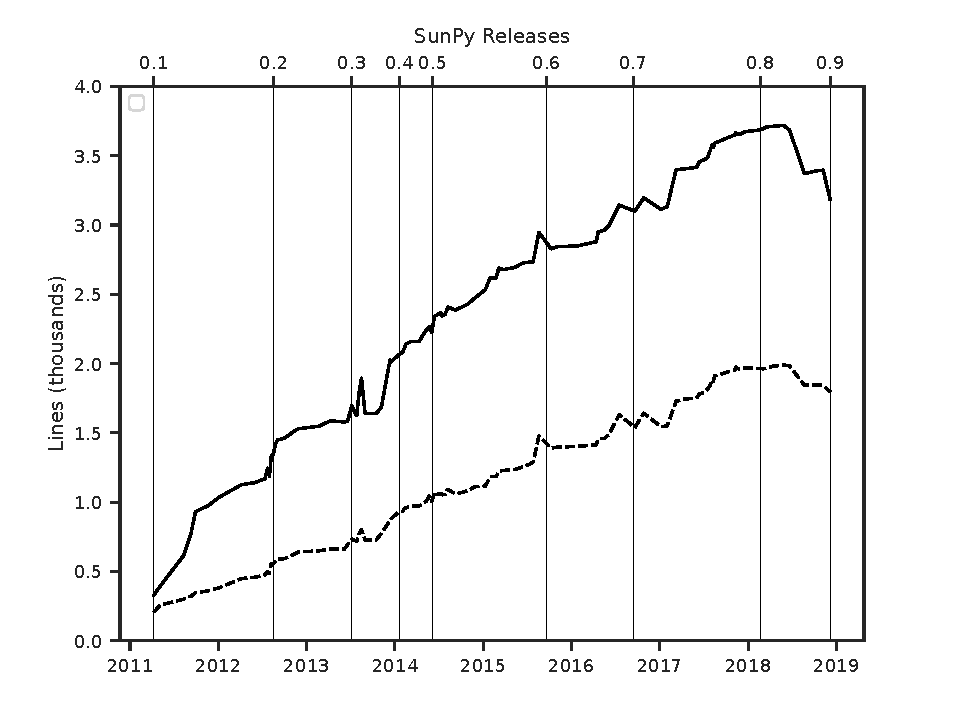
\includegraphics[width=45mm]{figures/sunpy_history.pdf} &
  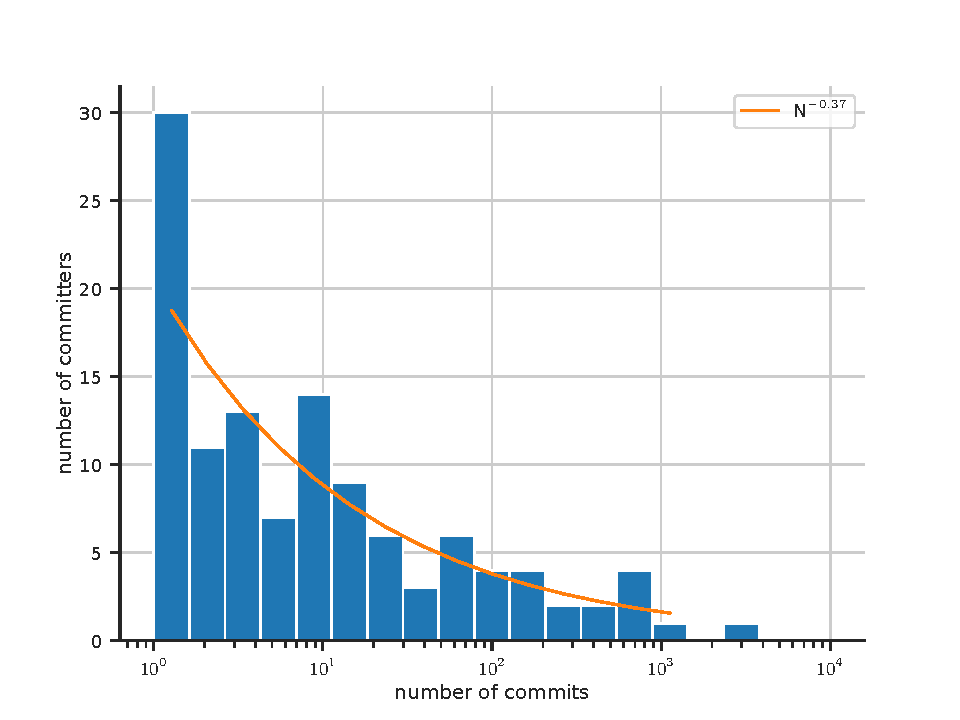
\includegraphics[width=45mm]{figures/busfactor_plot.pdf} &   
  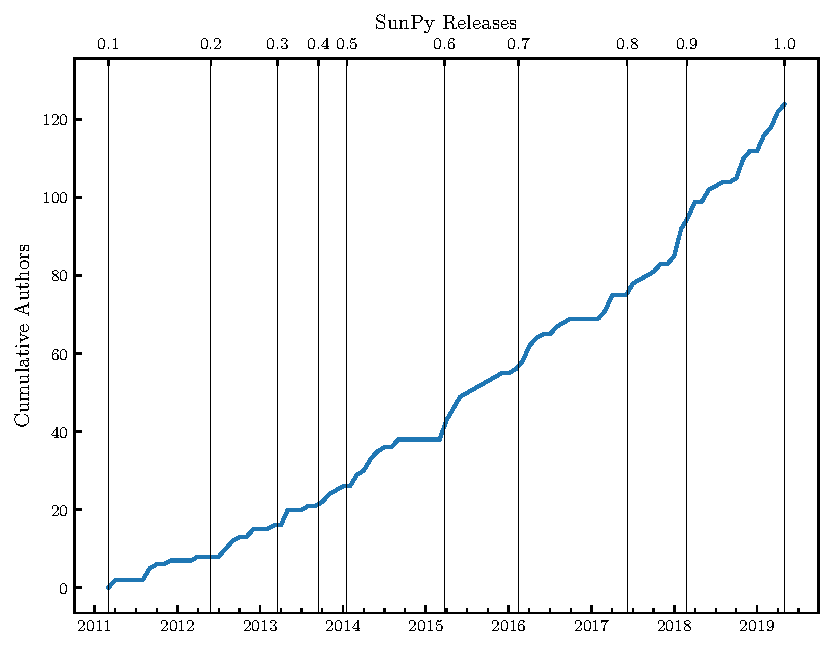
\includegraphics[width=45mm]{figures/cumulative_authors.pdf} \\
(a) & (b) & (c) \\
\end{tabular}
\caption{(a) The }
\label{fig:image2}
\end{figure}

